%% Compilado con TeX Live. Plantilla oficial Posgrado-UNI, marzo 2026.
\documentclass[a4paper,twocolumn]{article}
\usepackage[utf8]{inputenc}
\usepackage[T1]{fontenc}
\usepackage[spanish,es-nodecimaldot]{babel}
\usepackage[margin={1.5cm,2cm},columnsep=1cm]{geometry}
\usepackage{mathptmx,authblk,orcidlink,abstract,graphicx,caption,booktabs,amsmath,multirow,array}
\usepackage{microtype}
\usepackage{xurl}
\hypersetup{hidelinks,pdftitle={Marco analítico reproducible y auditable para dimensionar memoria de KV cache},pdfauthor={César Lara Ávila},pdfsubject={Artículo metodológico de inteligencia artificial},pdfkeywords={KV cache, GQA, SWA, MLA, contexto largo, dimensionamiento}}
\captionsetup{font=small,margin=0.05\linewidth}
\addto\captionsspanish{\renewcommand{\tablename}{Tabla}}
\setlength{\emergencystretch}{2em}

\title{Marco analítico reproducible y auditable para dimensionar memoria de KV cache en arquitecturas de atención de contexto largo\\[2ex]
A Reproducible and Auditable Analytical Framework for Sizing KV-Cache Memory in Long-Context Attention Architectures}

\author[1,\orcidlink{0009-0003-8564-615X},*]{César Lara Ávila}
\affil[1]{Facultad de Ciencias, Universidad Nacional de Ingeniería, Av. Túpac Amaru 210, Rímac, Lima 15333, Perú}
\affil[*]{Autor de correspondencia: César Lara Ávila (claraa@uni.edu.pe)}
\date{}

\begin{document}
\twocolumn[\maketitle
\begin{onecolabstract}
La memoria de claves y valores (KV cache) es una restricción central en la inferencia autoregresiva de modelos de lenguaje con contexto largo. Este trabajo presenta un marco analítico reproducible y auditable para dimensionar KV cache en atención multi-head (MHA), grouped-query attention (GQA), sliding-window attention (SWA) y una aproximación de cache latente inspirada en MLA. La contribución combina una ecuación unificada, factores adimensionales componibles y una formulación inversa que calcula la longitud de contexto admisible bajo un presupuesto de memoria. Se evaluaron 71 configuraciones entre $4\,096$ y $1\,048\,576$ tokens y cinco invariantes automatizados. Para 32 capas, dimensión $4\,096$, FP16 y $1\,048\,576$ tokens, MHA requiere 549.756 GB; GQA con 8 de 32 KV heads, 137.439 GB; SWA con ventana $8\,192$, 4.295 GB; y la aproximación latente de rango 512, 68.719 GB. Con un presupuesto lógico de 24 GB, el contexto completo admisible pasa de $45\,776$ tokens en MHA a $183\,105$ en GQA-8 y $366\,210$ en la aproximación latente. El marco está implementado en Attention AI Lab mediante API validada, escenarios versionados, reportes y pruebas. Una validación física mínima en PyTorch confirma las tendencias. Los resultados son estimaciones lógicas y no sustituyen perfiles de GPU.\\

\noindent\textbf{Palabras clave}: KV cache, contexto largo, atención multi-head, GQA, SWA, dimensionamiento reproducible.
\vspace{3ex}
\end{onecolabstract}
\renewcommand{\abstractname}{Abstract}
\begin{onecolabstract}
Key-value caching is a central constraint in autoregressive inference with long-context language models. This paper presents a reproducible and auditable analytical framework for sizing KV-cache memory under multi-head attention (MHA), grouped-query attention (GQA), sliding-window attention (SWA), and a latent-cache approximation inspired by MLA. The contribution combines a unified equation, composable dimensionless factors, and an inverse formulation that computes admissible context length under a memory budget. We evaluated 71 configurations from $4\,096$ to $1\,048\,576$ tokens and five automated invariants. For 32 layers, dimension $4\,096$, FP16 precision, and a $1\,048\,576$-token context, MHA requires 549.756 GB; GQA with 8 of 32 KV heads requires 137.439 GB; SWA with an $8\,192$-token window requires 4.295 GB; and the rank-512 latent approximation requires 68.719 GB. Under a logical 24 GB budget, admissible full context grows from $45\,776$ tokens with MHA to $183\,105$ with GQA-8 and $366\,210$ with the latent approximation. The framework is implemented in Attention AI Lab through a validated API, versioned scenarios, reports, and tests. A minimal PyTorch memory profile confirms the predicted trend. Values describe logical storage and do not replace GPU profiling.\\

\noindent\textbf{Keywords}: KV cache, long context, multi-head attention, grouped-query attention, sliding-window attention, reproducible sizing.
\vspace{3ex}
\end{onecolabstract}
]

\section{Introducción}
Los modelos Transformer establecieron la atención multi-head como componente central de los modelos de lenguaje modernos \cite{vaswani2017attention}. Durante la generación autoregresiva, las claves y valores asociados con los tokens ya procesados se almacenan para evitar recomputación. Esta KV cache reduce cálculo redundante, pero su almacenamiento lógico crece con la longitud de contexto, el número de capas, el lote, la dimensión almacenada y la precisión numérica \cite{shazeer2019fast,pope2022efficiently}. En contextos extensos, este estado puede convertirse en una restricción de capacidad antes de considerar latencia o throughput.

Las optimizaciones recientes actúan sobre distintos niveles del problema, desde cambios arquitectónicos y cuantización hasta eviction, paging, offloading y scheduling. El presente trabajo se concentra en una etapa previa a esas optimizaciones de ejecución: el dimensionamiento lógico y reproducible del payload de KV cache. El objetivo no es predecir memoria GPU ni rendimiento end-to-end, sino disponer de una representación compacta que permita comparar configuraciones bajo supuestos explícitos y vincular los cálculos con artefactos reproducibles.

\subsection{Trabajo relacionado y posicionamiento}
Las técnicas recientes de reducción de KV cache actúan sobre diferentes ejes. Multi-query attention comparte keys y values entre query heads, y GQA introduce un número intermedio de KV heads \cite{shazeer2019fast,ainslie2023gqa}. Cross-Layer Attention extiende el sharing entre capas \cite{brandon2024crosslayer}. Otra línea reduce la dimensión almacenada mediante representaciones low-rank o latentes, como MLA en DeepSeek-V2 y métodos de compresión low-rank como Palu \cite{deepseek2024v2,chang2025palu}. Estas arquitecturas motivan abstraer por separado la dimensión cacheada y el contexto efectivo, aunque sus implementaciones contienen estructura adicional que no puede reducirse a una sola razón escalar.

La compresión también puede actuar sobre el eje temporal o la precisión. H2O retiene heavy hitters y tokens recientes, StreamingLLM mantiene attention sinks junto con una ventana reciente y DuoAttention aplica full cache solo a retrieval heads \cite{zhang2023h2o,xiao2024streamingllm,xiao2025duoattention}. En cuantización, KIVI muestra que keys y values presentan propiedades diferentes, mientras SKVQ combina almacenamiento low-bit con una ventana de mayor precisión \cite{liu2024kivi,duanmu2024skvq}. Por ello, reducir $T_{\mathrm{eff}}$ o los bytes por valor es útil para contabilidad lógica, pero no describe por sí solo pérdida de calidad, metadatos ni overhead de kernels.

En sistemas de serving, el payload lógico tampoco determina la memoria físicamente utilizable. PagedAttention reduce desperdicio mediante paging y sharing de bloques, vAttention separa espacio virtual contiguo de backing físico y KV-Compress muestra que una tasa teórica de compresión puede no materializarse de forma proporcional cuando el layout introduce fragmentación \cite{kwon2023efficient,prabhu2025vattention,rehg2024kvcompress}. Evaluaciones de serving como Rethinking KV Compression encuentran además que reducir memoria no garantiza una mejora equivalente de throughput o latencia \cite{gao2025rethinking}. Estudios recientes de calidad muestran que determinadas instrucciones pueden degradarse de forma desigual bajo compresión \cite{chen2026pitfalls}.

Finalmente, LIFE modela analíticamente el rendimiento de inferencia a partir de operadores y especificaciones de hardware, mientras KV Pareto estudia empíricamente fronteras entre memoria total y accuracy para combinaciones de optimizaciones \cite{patwari2025life,gokhale2026kvpareto}. Otros trabajos distribuyen budgets de retención entre capas, y una taxonomía reciente organiza la gestión de KV cache en niveles de token, modelo y sistema \cite{li2024xkv,li2024kvsurvey}. El presente trabajo persigue un objetivo más acotado: proporcionar una capa de dimensionamiento lógico de capacidad para configuraciones seleccionadas, con una representación común, cálculo directo e inverso y trazabilidad reproducible entre ecuaciones, implementación, datos regenerables y pruebas. Este nivel de análisis complementa, en lugar de sustituir, modelos de rendimiento, técnicas de compresión y sistemas de gestión física de memoria.

\subsection{Objetivo y contribuciones}
La literatura reciente integra mecanismos de reducción y gestión de KV cache desde perspectivas arquitectónicas, algorítmicas y de sistemas. Sin embargo, para una etapa preliminar de capacity planning sigue siendo útil una representación compacta que permita responder de forma reproducible cuánto payload lógico requiere una configuración, qué factores explican una reducción, qué mecanismos pueden componerse bajo supuestos explícitos y qué contexto satisface un presupuesto reservado a KV cache. El objetivo de este trabajo es proporcionar esa capa de dimensionamiento y vincularla con un artefacto ejecutable y auditable, sin interpretar las estimaciones lógicas como mediciones de GPU.

Las contribuciones del trabajo son cuatro. Primero, se define un modelo compacto de almacenamiento lógico de KV cache para MHA, GQA, una variante de sliding-window attention y una aproximación de cache latente mediante variables comunes de contexto efectivo, dimensión cacheada, profundidad, lote y precisión. Segundo, se introducen factores relativos para comparar y componer reducciones compatibles bajo supuestos explícitos, y el mismo modelo se utiliza en forma inversa para calcular contexto admisible bajo un presupuesto lógico reservado al payload de KV cache. Tercero, se evalúan 71 configuraciones y cinco invariantes científicos mediante artefactos regenerables y resultados deterministas. Cuarto, Attention AI Lab vincula la formulación con cálculos canónicos, contratos, escenarios, datos y pruebas automatizadas, proporcionando trazabilidad desde las ecuaciones hasta los artefactos científicos. Una comprobación empírica acotada de storage en CPU verifica la contabilidad elemental sin sustituir profiling de GPU \cite{lara2026attentionlab}.

\section{Materiales y métodos}
\subsection{Modelo analítico base}
Para un decodificador autoregresivo con $L$ capas, contexto efectivo $T_{\mathrm{eff}}$, lote $B$, dimensión cacheada por token $d_{\mathrm{cache}}$ y $s$ bytes por valor, la memoria decimal estimada es:
\begin{equation}\label{eq:base}
M_{\mathrm{KV}}=\frac{L\,T_{\mathrm{eff}}\,2\,d_{\mathrm{cache}}\,s\,B}{10^{9}}\quad [\mathrm{GB}].
\end{equation}
El factor 2 corresponde a keys y values. La Ecuación~\eqref{eq:base} modela almacenamiento lógico. No incluye pesos, activaciones temporales, buffers de kernels, alineamiento, fragmentación, páginas ni metadatos del runtime.

Para MHA, $T_{\mathrm{eff}}=T$ y $d_{\mathrm{cache}}=d$:
\begin{equation}\label{eq:mha}
M_{\mathrm{MHA}}=\frac{L\,T\,2\,d\,s\,B}{10^{9}}.
\end{equation}
La Ecuación~\eqref{eq:mha} define el baseline MHA utilizado en las comparaciones posteriores.

\subsection{Factores arquitectónicos}
Sea $h_q$ el número de query heads y $h_{kv}$ el número de KV heads. Bajo dimensión uniforme por head, GQA reduce la dimensión total almacenada en la razón:
\begin{equation}\label{eq:gqa}
M_{\mathrm{GQA}}=M_{\mathrm{MHA}}\frac{h_{kv}}{h_q},\qquad
R_{\mathrm{GQA}}=\frac{h_{kv}}{h_q}.
\end{equation}
La Ecuación~\eqref{eq:gqa} expresa la reducción proporcional producida al compartir claves y valores entre grupos de query heads.

En SWA, el contexto activo se limita a una ventana $W$:
\begin{equation}\label{eq:swa}
M_{\mathrm{SWA}}=\frac{L\,\min(T,W)\,2\,d\,s\,B}{10^{9}},\qquad
R_{\mathrm{SWA}}=\frac{\min(T,W)}{T}.
\end{equation}
La Ecuación~\eqref{eq:swa} cuantifica la memoria cuando el contexto efectivo se limita a una ventana local. La formulación representa una ventana estrictamente local. Diseños con tokens globales o estados adicionales requieren términos complementarios.

Para una aproximación abstracta de cache latente que almacena, por token y por capa, dos representaciones de dimensión $r<d$, una asociada a claves y otra a valores:
\begin{equation}\label{eq:latent}
M_{\mathrm{LAT}}=\frac{L\,T\,2\,r\,s\,B}{10^{9}},\qquad
R_{\mathrm{LAT}}=\frac{r}{d}.
\end{equation}
La Ecuación~\eqref{eq:latent} modela el almacenamiento de las dos representaciones latentes por token y por capa. El factor $2r$ representa explícitamente ambas variables latentes. Esta formulación es una aproximación de almacenamiento inspirada en MLA, no una reproducción exacta de DeepSeek-V2: una implementación concreta puede emplear una representación comprimida conjunta y conservar componentes posicionales, proyecciones u otros estados adicionales \cite{deepseek2024v2}.

\subsection{Factorización y composición}
Al comparar una variante contra un baseline MHA con iguales $L$, $B$ y precisión, la razón general es:
\begin{equation}\label{eq:ratio}
R=\frac{M}{M_{\mathrm{MHA}}}=\frac{T_{\mathrm{eff}}}{T}\frac{d_{\mathrm{cache}}}{d}.
\end{equation}
La Ecuación~\eqref{eq:ratio} separa la reducción debida al contexto efectivo de la reducción debida a la dimensión cacheada. Cuando dos mecanismos actúan sobre factores distintos, sus razones pueden componerse. Por ejemplo, una aproximación GQA+SWA usa:
\begin{equation}\label{eq:compose}
R_{\mathrm{GQA+SWA}}=\frac{h_{kv}}{h_q}\frac{\min(T,W)}{T}.
\end{equation}
Una reducción de precisión multiplica además por $s/s_0$. Esta composición describe requisitos lógicos; no asegura que una arquitectura concreta preserve calidad, latencia o compatibilidad de kernels.

\subsection{Inversión por presupuesto de memoria}
Para atención de contexto completo, un presupuesto $G$ en GB permite despejar la longitud máxima:
\begin{equation}\label{eq:budget}
T_{\max}=\left\lfloor\frac{G\,10^{9}}{L\,2\,d_{\mathrm{cache}}\,s\,B}\right\rfloor.
\end{equation}
En MHA, $d_{\mathrm{cache}}=d$; en GQA, $d_{\mathrm{cache}}=d(h_{kv}/h_q)$; y en la aproximación latente, $d_{\mathrm{cache}}=r$. Para SWA, el costo se estabiliza cuando $T\ge W$, por lo que la pregunta relevante es si la ventana cabe en el presupuesto, no el contexto global máximo.

\subsection{Diseño experimental}
El escenario base usa 32 capas, dimensión $4\,096$, 32 query heads, lote 1 y FP16. Se evaluaron contextos de $4\,096$, $8\,192$, $16\,384$, $32\,768$, $65\,536$, $131\,072$, $262\,144$, $524\,288$ y $1\,048\,576$ tokens. GQA empleó $h_{kv}\in\{32,16,8,4,2,1\}$; SWA, $W\in\{2\,048,4\,096,8\,192,16\,384,32\,768\}$; y la cache latente, $r\in\{128,256,512,1024\}$. La precisión consideró FP32, FP16, BF16, INT8 e INT4 con 4, 2, 2, 1 y 0.5 bytes por valor.

El conjunto incluye 71 estimaciones: 36 para contexto, 15 para parámetros arquitectónicos y 20 para precisión. INT8 e INT4 representan almacenamiento ideal; no incluyen escalas, zero-points, agrupamiento ni efectos de calidad \cite{liu2024kivi}.

\subsection{Métricas y criterios de verificación}
Se reportan memoria en GB decimales, razón $R=M/M_{\mathrm{MHA}}$, reducción $100(1-R)$ y $T_{\max}$ bajo presupuestos de 24, 48 y 80 GB. La implementación se verifica con cinco invariantes: linealidad de MHA respecto a $T$; razón GQA igual a $h_{kv}/h_q$; saturación SWA para $T\ge W$; razón latente igual a $r/d$; y consumo INT8 igual a la mitad de FP16 bajo parámetros idénticos.

\subsection{Validación física mínima en PyTorch}
Como comprobación física acotada, se materializaron tensores FP16 en CPU con PyTorch 2.10.0 usando la forma $[L,2,B,T,d_{\mathrm{cache}}]$. Cada escenario se ejecutó tres veces en un subproceso nuevo; después de importar PyTorch se midió la memoria residente (RSS), se escribió el tensor completo para comprometer sus páginas y se compararon la Ecuación~\eqref{eq:base}, los bytes de \texttt{untyped\_storage().nbytes()} y la mediana del incremento de RSS. Se usaron dos configuraciones reducidas: MHA con $L=4$, $T=8\,192$ y $d_{\mathrm{cache}}=1\,024$; y GQA-4/16 con $d_{\mathrm{cache}}=256$. La escala evita consumir recursos excesivos y permite comprobar tanto el almacenamiento lineal como la razón esperada de un cuarto. Esta prueba no incluye pesos, kernels de atención ni memoria CUDA, por lo que no constituye un benchmark de GPU.

\section{Desarrollo}
\subsection{Implementación en Attention AI Lab}
El marco se implementó en Attention AI Lab v1.2.0, una aplicación full-stack con backend FastAPI/Pydantic y frontend React/TypeScript \cite{lara2026attentionlab}. El servicio determinista central se expone mediante \texttt{/api/llm/estimate}. El contrato acepta entre 1 y 256 capas, dimensión de 64 a $32\,768$, entre 1 y 256 query heads y KV heads, rango latente de 1 a $8\,192$, contexto de 128 a $1\,048\,576$ tokens, lote de 1 a 128 y precisiones FP32, FP16, BF16, INT8 e INT4.

El servicio principal calcula MHA, GQA y cache latente. SWA se obtiene en la capa de validación reproducible aplicando $\min(T,W)$ sobre el resultado MHA. Esta separación se mantiene explícita para no atribuir al contrato público una salida que todavía se deriva en el script de reporte. El estudio tampoco usa los proxies didácticos de perplejidad y tokens por segundo incluidos en la interfaz, porque no son mediciones calibradas.

La aplicación puede ejecutarse sin GPU, sin API keys y sin servicios externos obligatorios. Un Docker multi-stage compila el frontend y sirve API, interfaz y documentación OpenAPI en el puerto 7860. Una demostración interactiva está disponible en \url{https://kapumota-attentio-ai-lab.hf.space/}. El Space constituye un entorno demostrativo en evolución y puede recibir actualizaciones posteriores; por ello, permite inspeccionar la interfaz y el contrato, pero no sustituye la referencia inmutable usada para reproducir el estudio. El paquete del artículo conserva CSV, figuras y script independientes.

\subsection{Trazabilidad del artefacto}
La Tabla~\ref{tab:traceability} vincula cada afirmación computacional con un artefacto verificable del repositorio.

\begin{table*}[!ht]
\centering\footnotesize
\caption{Trazabilidad entre formulación, implementación y evidencia. Fuente: elaboración propia a partir de Attention AI Lab v1.2.0.}\label{tab:traceability}
\begin{tabular}{>{\raggedright\arraybackslash}p{0.28\textwidth}>{\raggedright\arraybackslash}p{0.44\textwidth}>{\raggedright\arraybackslash}p{0.18\textwidth}}
\toprule
Artefacto & Función en el estudio & Evidencia \\
\midrule
\texttt{llm\_metrics.py} & Implementa bytes por precisión y las ecuaciones lógicas para MHA, GQA y cache latente. & Salidas numéricas deterministas. \\
\texttt{contracts.py} & Restringe dominios de capas, dimensión, heads, rango, contexto, lote y precisión. & Validación Pydantic del contrato. \\
\path{examples/kv-cache-validation-scenarios.json} & Versiona cuatro escenarios de referencia entre $32\,768$ y $1\,048\,576$ tokens. & Configuración auditable. \\
\path{scripts/generate-kv-cache-validation-report.py} & Ejecuta el servicio, deriva SWA y genera un reporte Markdown. & Tabla reproducible. \\
\path{apps/api/tests/test_kv_cache_validation.py} & Verifica linealidad, razones GQA/SWA/latente y finitud del escenario de $1\,048\,576$ tokens. & Cinco pruebas de regresión. \\
\path{profile_pytorch_memory.py} & Materializa dos tensores FP16, mide storage y RSS en subprocesos nuevos. & \path{data/pytorch_memory_profile.csv}. \\
\texttt{QUALITY\_GATE.md} & Centraliza Pytest, chequeo TypeScript, limpieza y validación del Space. & Comando \texttt{make validate}. \\
\url{https://kapumota-attentio-ai-lab.hf.space/} & Proporciona una demostración interactiva del estimador y de los módulos educativos. & Despliegue demostrativo mutable. \\
\bottomrule
\end{tabular}
\end{table*}

\subsection{Protocolo reproducible}
El protocolo consta de cinco pasos: (1) fijar supuestos y escenarios; (2) ejecutar el estimador determinista; (3) exportar CSV y figuras; (4) comprobar invariantes; y (5) ejecutar el perfil físico mínimo de PyTorch. El quality gate exige pruebas backend, compilación y chequeo TypeScript, revisión documental y validación opcional del despliegue público. Esto no valida fidelidad física, pero reduce errores de transcripción, cambios silenciosos de fórmula y discrepancias entre documentación y código.

\section{Resultados y discusión}
\subsection{Escalamiento con la longitud de contexto}
La Figura~\ref{fig:context} muestra el barrido de $4\,096$ a $1\,048\,576$ tokens. MHA, GQA y la aproximación latente crecen linealmente con $T$ y conservan razones constantes. SWA se estabiliza al alcanzar la ventana de $4\,096$ tokens.

\begin{figure*}[!ht]
\centering
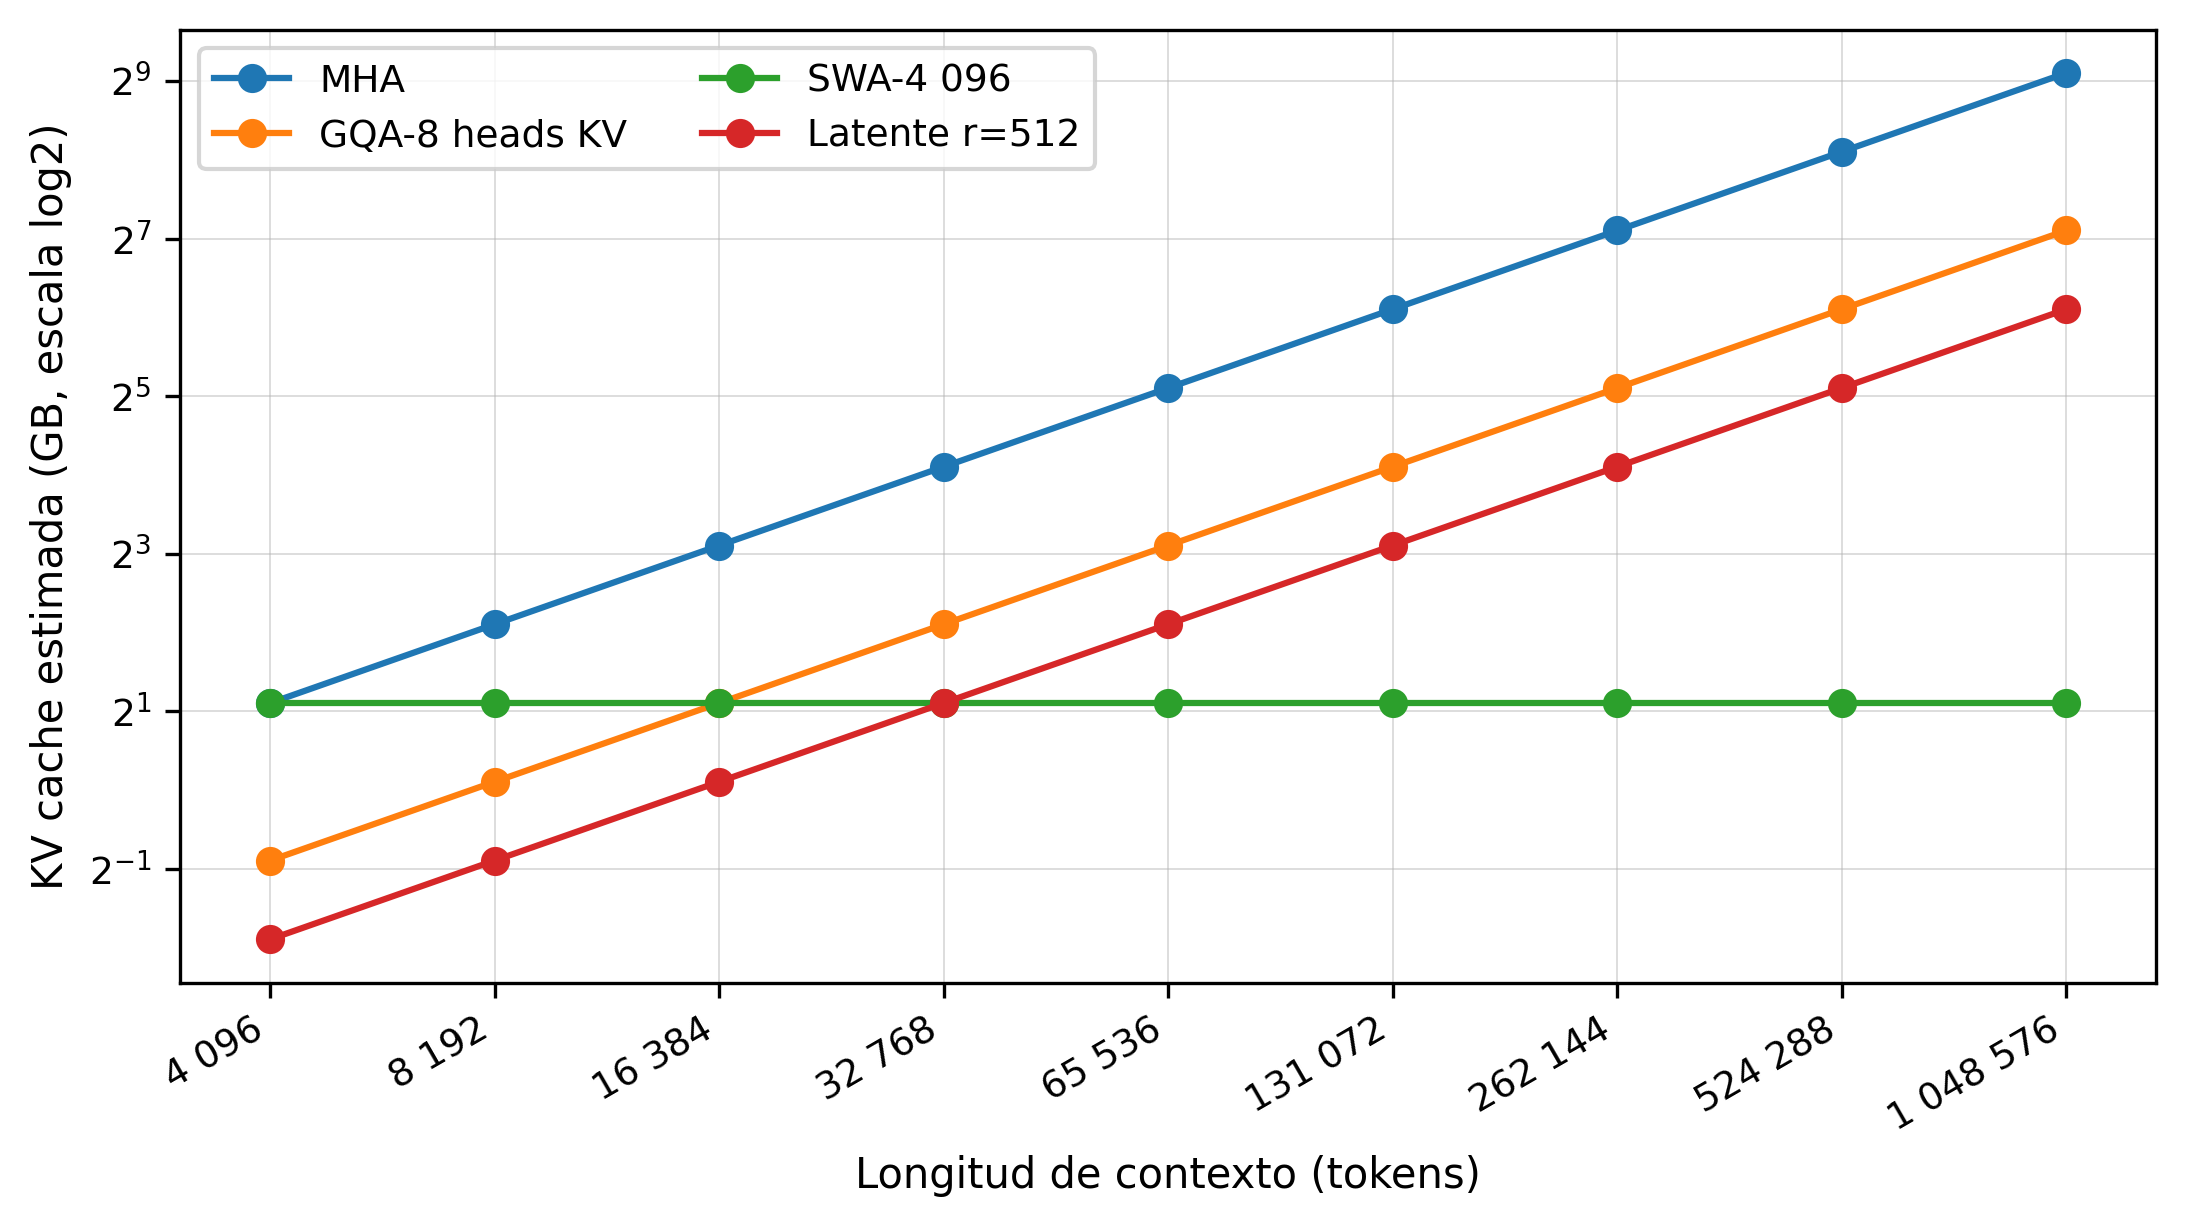
\includegraphics[width=0.88\linewidth]{figures/context_sweep.png}
\caption{Memoria estimada de KV cache al variar la longitud de contexto. Supuestos: 32 capas, dimensión $4\,096$, FP16, lote 1, GQA con 8 de 32 KV heads, SWA con ventana $4\,096$ y cache latente de rango 512. Fuente: elaboración propia.}\label{fig:context}
\end{figure*}

La Tabla~\ref{tab:scenarios} separa las cuatro familias para evitar interpretar SWA y cache latente como una misma salida. En $1\,048\,576$ tokens, MHA requiere 549.756 GB. GQA-8 reduce 75\%, la cache latente de rango 512 reduce 87.5\% y SWA-$8\,192$ reduce 99.219\% respecto al baseline MHA. Esta última reducción se obtiene al renunciar a atención directa sobre tokens fuera de la ventana local.

\begin{table*}[!ht]
\centering\small
\caption{Escenarios representativos de memoria lógica estimada. Valores en GB decimales. Fuente: elaboración propia.}\label{tab:scenarios}
\begin{tabular}{lrrrrr}
\toprule
Escenario & Contexto & MHA & GQA & SWA & Latente \\
\midrule
MHA $32\,768$, 32 KV heads & 32 768 & 17.180 & 17.180 & 2.147 & 2.147 \\
GQA $65\,536$, 8 de 32 KV heads & 65 536 & 34.360 & 8.590 & 2.147 & 4.295 \\
SWA $131\,072$, ventana $4\,096$ & 131 072 & 68.719 & 17.180 & 2.147 & 8.590 \\
Contexto $1\,048\,576$, ventana $8\,192$, rango 512 & 1 048 576 & 549.756 & 137.439 & 4.295 & 68.719 \\
\bottomrule
\end{tabular}
\end{table*}

\subsection{Sensibilidad arquitectónica a 131 072 tokens}
La Figura~\ref{fig:ratios} confirma que GQA depende de $h_{kv}/h_q$. Con 16, 8, 4 y 1 KV heads sobre 32 query heads, las razones son 0.5, 0.25, 0.125 y 0.03125. La reducción permanece constante al cambiar $T$ si las demás variables no cambian.

\begin{figure*}[!ht]
\centering
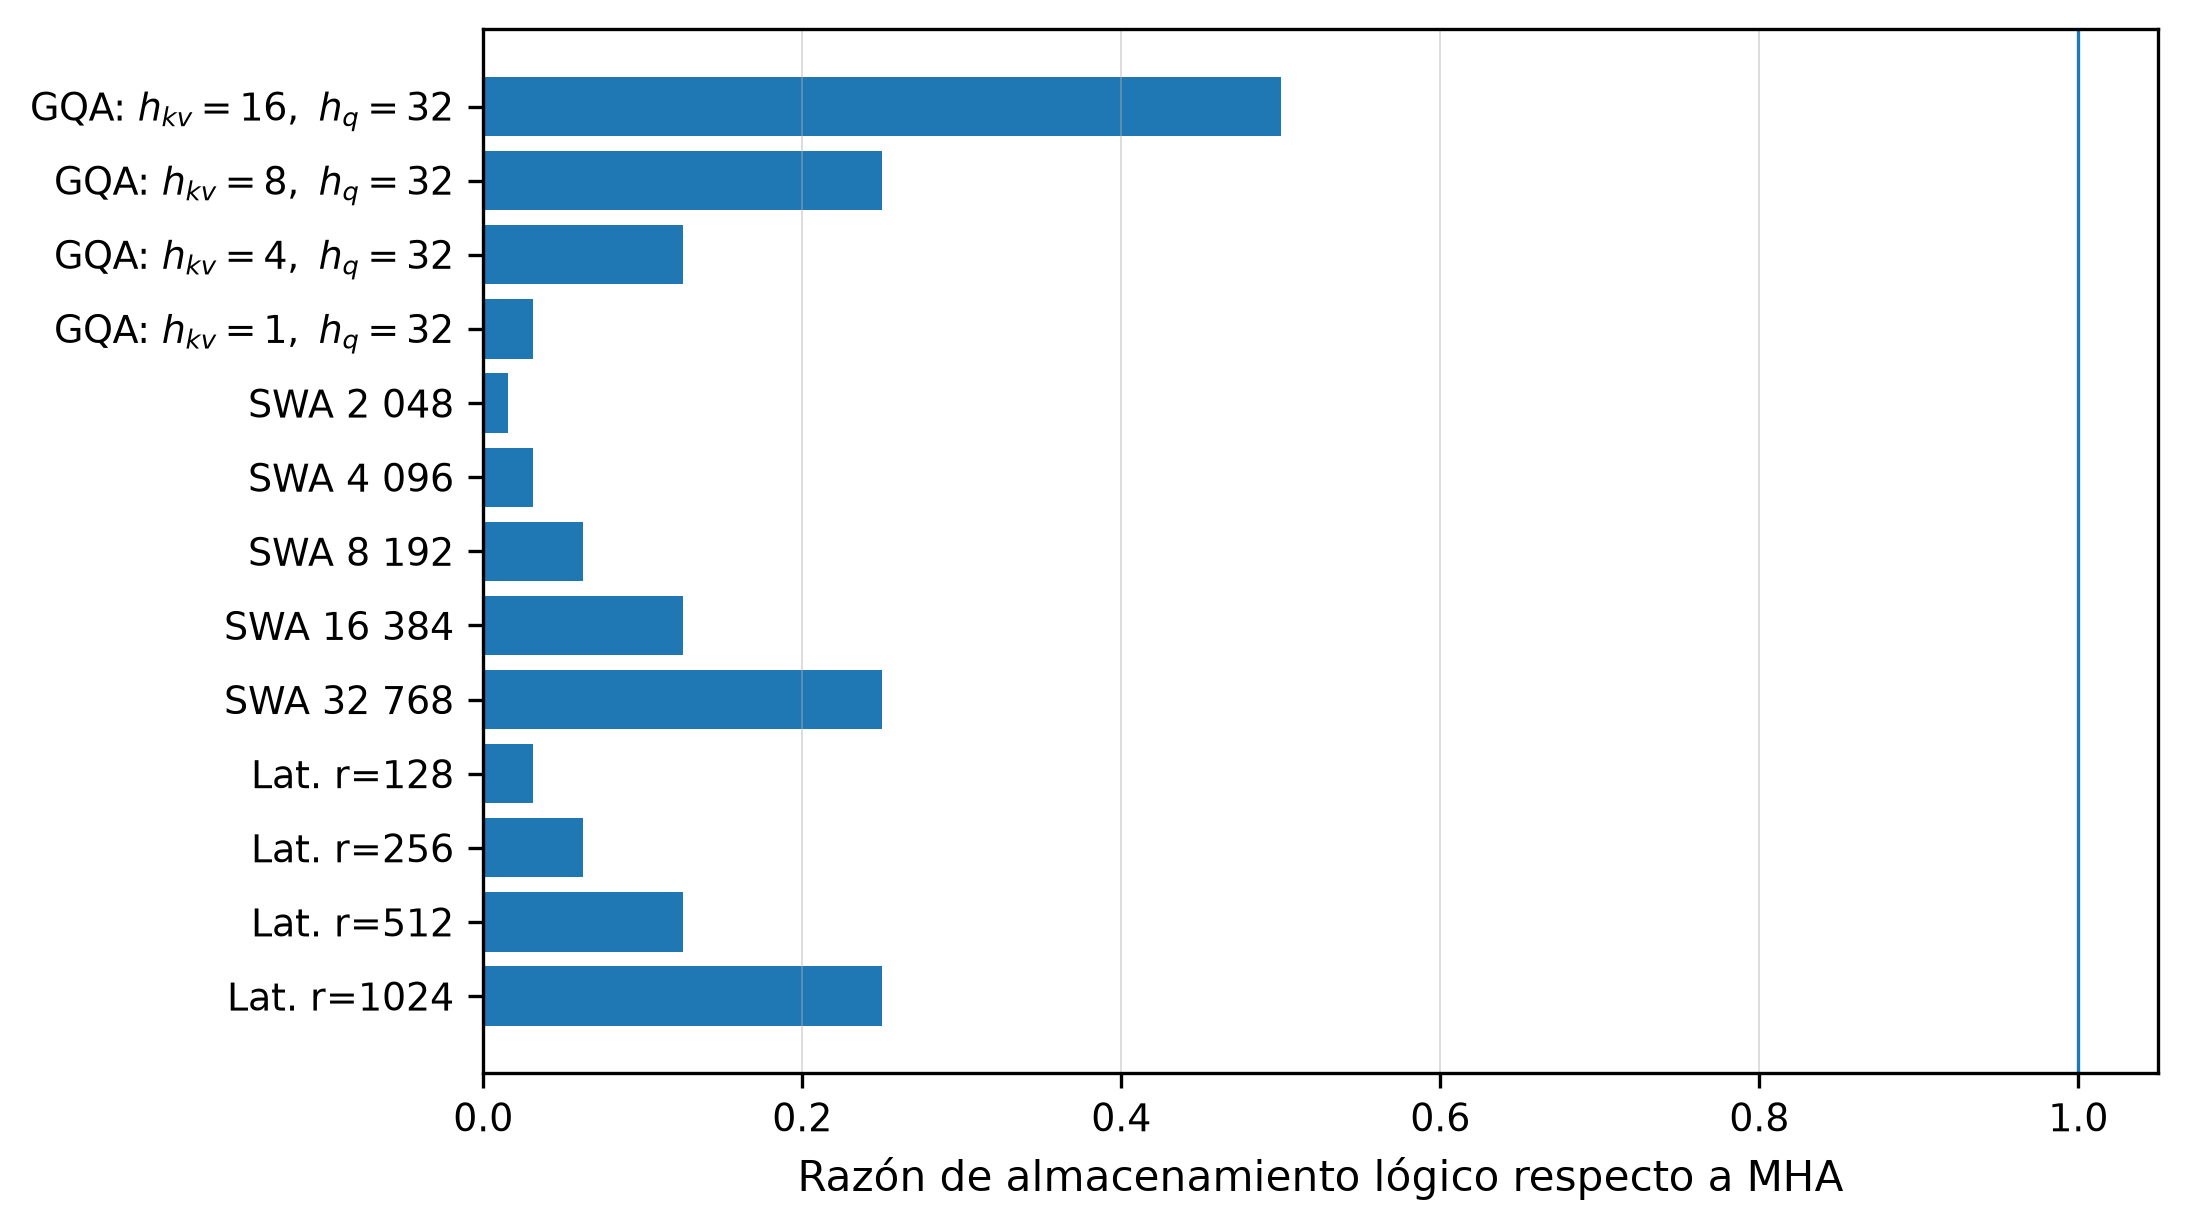
\includegraphics[width=0.88\linewidth]{figures/ratios_128k.png}
\caption{Razón de memoria respecto a MHA para configuraciones a $131\,072$ tokens. ``Lat.'' corresponde a cache latente. Fuente: elaboración propia.}\label{fig:ratios}
\end{figure*}

SWA-$4\,096$ también produce $R=0.03125$ a $131\,072$, igual que GQA con un KV head. La igualdad de memoria no implica equivalencia funcional: GQA conserva todo el contexto mediante compartición entre query heads, mientras SWA limita el historial activo. La cache latente produce razones 0.03125, 0.0625, 0.125 y 0.25 para rangos 128, 256, 512 y 1024.

La composición de la Ecuación~\eqref{eq:compose} ofrece un escenario de planeamiento adicional. A $1\,048\,576$ tokens, GQA-8 con SWA-$8\,192$ reduce la cache lógica FP16 de 549.756 GB a 1.074 GB. Si además se representa cada valor con 1 byte, el valor ideal es 0.537 GB. Estas cifras no describen una implementación ni su calidad; muestran cómo los factores independientes pueden detectar órdenes de magnitud antes del despliegue.

\subsection{Efecto de la precisión}
La Figura~\ref{fig:precision} muestra escalamiento lineal con bytes por valor. Para MHA a $131\,072$ tokens, FP32 requiere 137.439 GB; FP16 y BF16, 68.719 GB; INT8, 34.360 GB; e INT4, 17.180 GB.

\begin{figure*}[!ht]
\centering
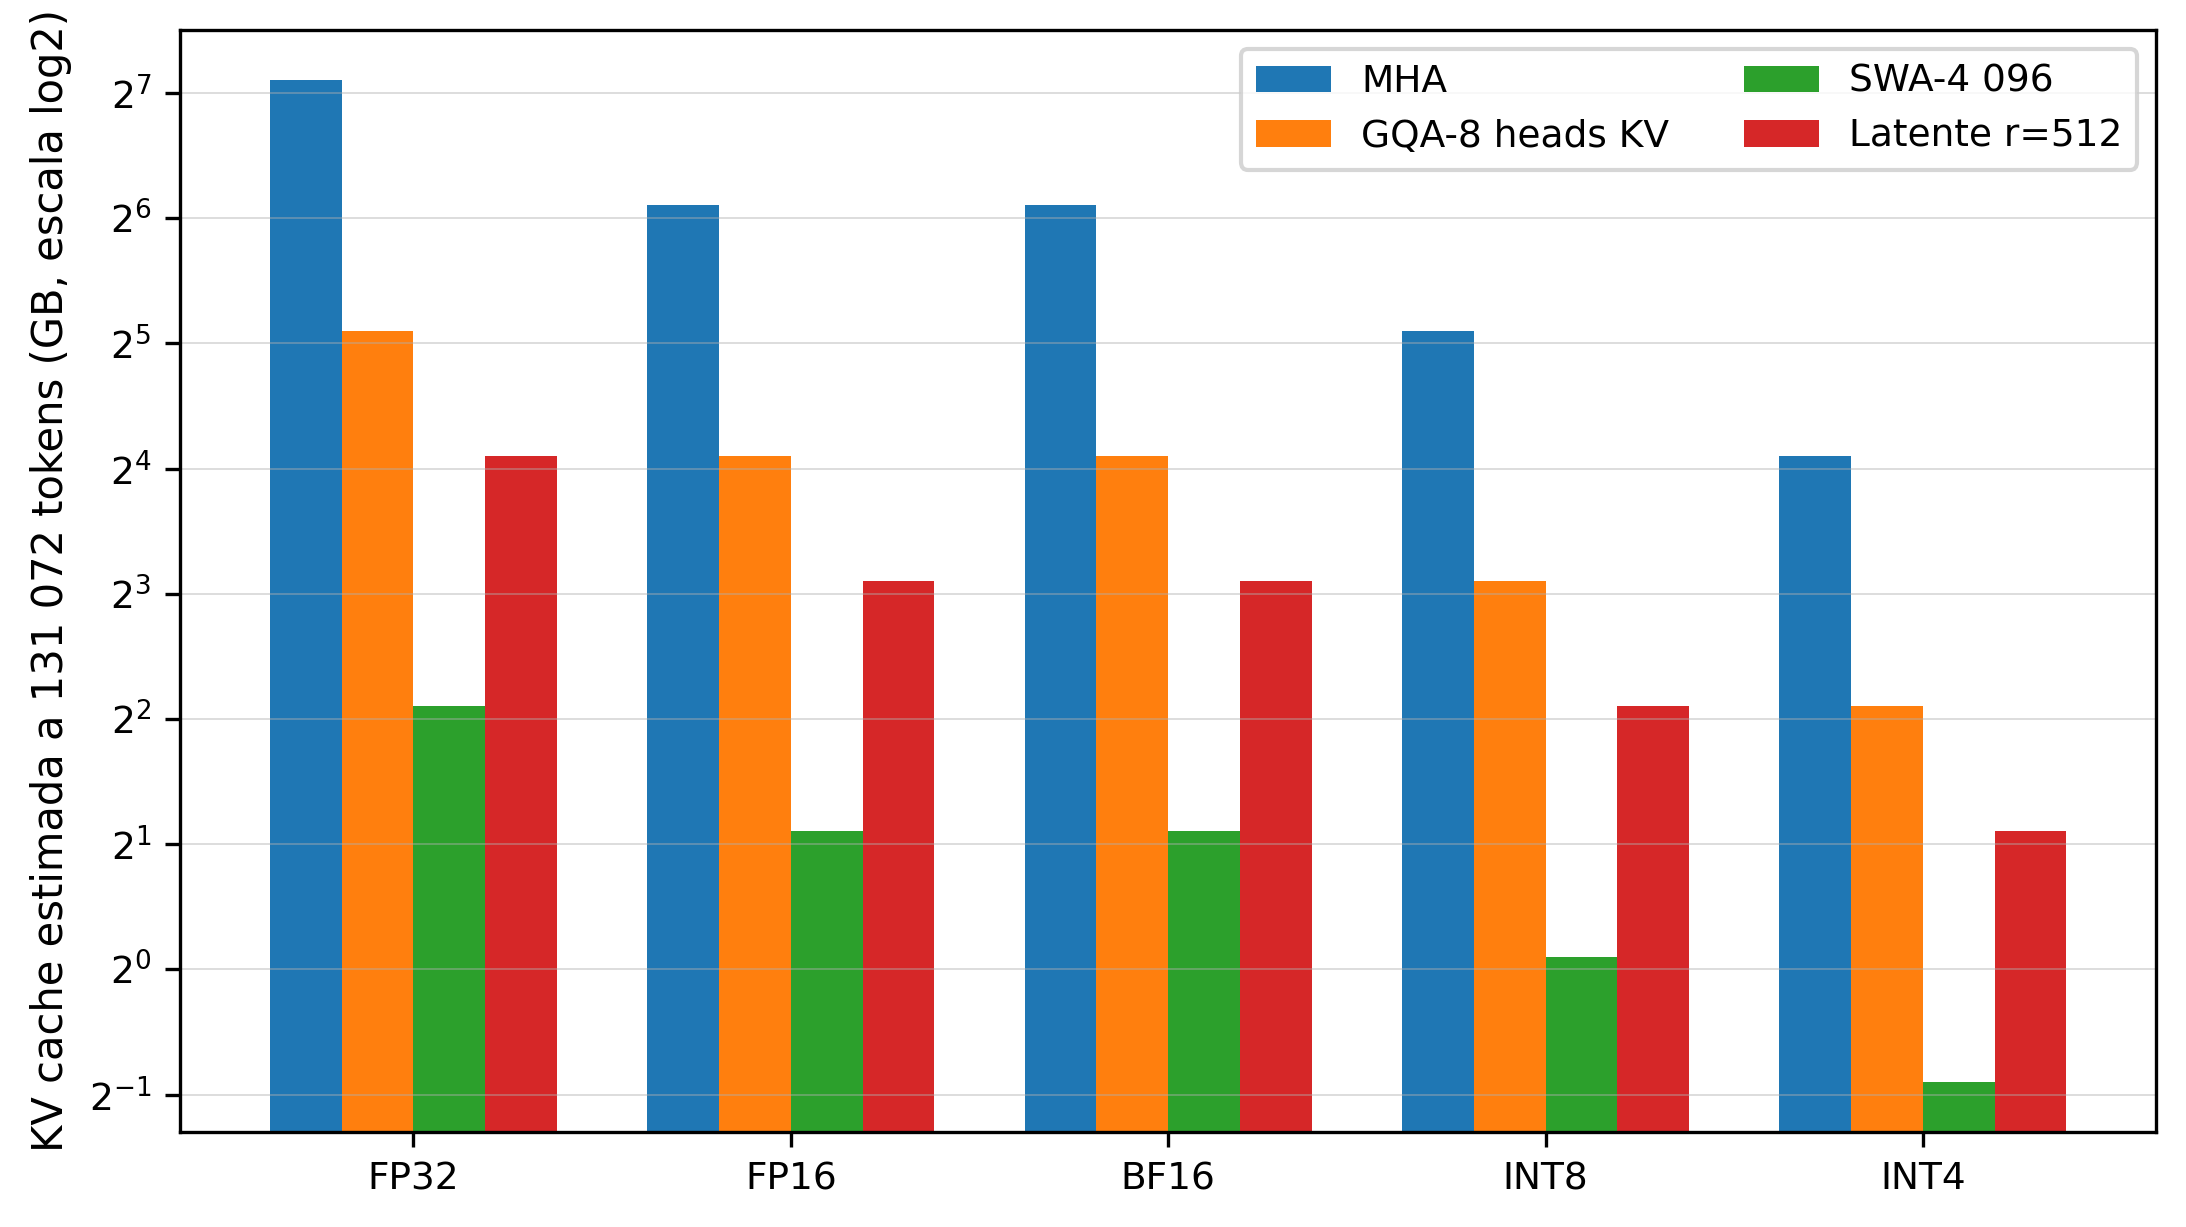
\includegraphics[width=0.88\linewidth]{figures/precision_128k.png}
\caption{Sensibilidad a la precisión para $131\,072$ tokens. INT8 e INT4 representan almacenamiento ideal y omiten metadatos de cuantización. Fuente: elaboración propia.}\label{fig:precision}
\end{figure*}

La cuantización puede multiplicar reducciones de GQA o SWA, pero su efecto práctico depende de granularidad, escalas, outliers y kernels. KIVI muestra que keys y values pueden requerir tratamientos distintos, por lo que reducir bytes no basta para caracterizar calidad ni rendimiento \cite{liu2024kivi}.

\subsection{Contexto admisible bajo presupuesto}
La Ecuación~\eqref{eq:budget} transforma el estimador en una herramienta de decisión. La Tabla~\ref{tab:budget} considera memoria reservada exclusivamente para KV cache. Con 24 GB, MHA admite $45\,776$ tokens de contexto completo; GQA-8, $183\,105$; y rango latente 512, $366\,210$. En una GPU de 80 GB, los límites lógicos son $152\,587$, $610\,351$ y $1\,220\,703$ tokens. En producción, el presupuesto disponible debe descontar pesos, activaciones y runtime.

\begin{table}[!ht]
\centering\small
\caption{Contexto completo máximo por presupuesto lógico de KV cache. Modelo base FP16. Fuente: elaboración propia.}\label{tab:budget}
\begin{tabular}{rrrr}
\toprule
Presupuesto KV & MHA & GQA-8 & Latente $r=512$ \\
\midrule
24 GB & $45\,776$ & $183\,105$ & $366\,210$ \\
48 GB & $91\,552$ & $366\,210$ & $732\,421$ \\
80 GB & $152\,587$ & $610\,351$ & $1\,220\,703$ \\
\bottomrule
\end{tabular}
\end{table}

\subsection{Validación por invariantes}
La Tabla~\ref{tab:invariants} resume las pruebas. El error absoluto es cero dentro de la aritmética del script. Estas pruebas validan coherencia entre ecuaciones y código, no correspondencia con hardware.

\begin{table}[!ht]
\centering\small
\caption{Invariantes de la implementación. Fuente: elaboración propia.}\label{tab:invariants}
\begin{tabular}{lcc}
\toprule
Invariante & Esperado & Observado \\
\midrule
$M_{\mathrm{MHA}}(2T)/M_{\mathrm{MHA}}(T)$ & 2.000 & 2.000 \\
GQA $8/32$ heads & 0.250 & 0.250 \\
SWA $4\,096/131\,072$ & 0.03125 & 0.03125 \\
Latente $512/4096$ & 0.125 & 0.125 \\
INT8 / FP16 & 0.500 & 0.500 \\
\bottomrule
\end{tabular}
\end{table}

\subsection{Validación física mínima en PyTorch}
La Tabla~\ref{tab:pytorch-profile} muestra que los bytes del storage de PyTorch coinciden exactamente con la predicción analítica en ambas configuraciones. Para MHA, la Ecuación~\eqref{eq:base} predijo 134.218 MB y la mediana del incremento de RSS fue 134.222 MB; para GQA-4/16, los valores fueron 33.554 y 33.559 MB. En ambos casos la diferencia física fue de $4\,096$ bytes, equivalente a una página de memoria, y el error relativo respecto al modelo fue menor que 0.013\%. La razón observada GQA/MHA fue 0.25. Este resultado respalda la contabilidad elemental de almacenamiento y la tendencia de reducción, pero no valida overheads de un runtime de inferencia ni comportamiento en GPU.

\begin{table}[!ht]
\centering\scriptsize
\caption{Perfil mínimo de memoria con PyTorch 2.10.0 en CPU; tres ejecuciones por escenario. Valores en MB decimales. Fuente: elaboración propia.}\label{tab:pytorch-profile}
\begin{tabular}{lrrrr}
\toprule
Escenario & Analítico & Storage & RSS mediana & Error RSS \\
\midrule
MHA & 134.218 & 134.218 & 134.222 & 0.003\% \\
GQA-4/16 & 33.554 & 33.554 & 33.559 & 0.012\% \\
\bottomrule
\end{tabular}
\end{table}

\subsection{Discusión y amenazas a la validez}
El resultado principal no es una nueva variante de atención, sino una descomposición útil para planeamiento. GQA y cache latente producen factores constantes; SWA sustituye contexto global por una ventana acotada; y la precisión escala todas las familias. La formulación inversa evita limitar el análisis a tablas directas y permite preguntar qué contexto cabe en una restricción dada.

La trazabilidad del repositorio aporta una segunda dimensión de solidez: las ecuaciones están vinculadas con servicio, contrato, escenarios, reporte, pruebas y quality gate. El despliegue público facilita inspección, pero no se utiliza como evidencia de rendimiento. Tampoco se incluyen los proxies de velocidad o perplejidad de la interfaz.

La validación mínima confirma la asignación de tensores puros en CPU, pero la amenaza principal a la validez externa sigue siendo la diferencia entre esa memoria lógica y la memoria física de un sistema de inferencia completo. Frameworks de inferencia agregan alineamiento, fragmentación, páginas, buffers y cachés auxiliares. El costo total también contiene pesos y activaciones. Además, reducir KV heads, ventana, rango o precisión puede afectar calidad y latencia de manera dependiente del modelo y de la tarea. Finalmente, la aproximación latente omite componentes específicos de MLA. Por ello, los resultados son una cota de dimensionamiento y no una garantía de ejecución.

La siguiente fase debe calibrar un modelo $M_{\mathrm{fisico}}=\alpha M_{\mathrm{logico}}+M_{\mathrm{aux}}$ mediante perfiles PyTorch/CUDA en GPU y comparar error relativo en distintos runtimes. Una evaluación completa debería incorporar vLLM, memoria pico, latencia, throughput y calidad para obtener fronteras de Pareto.

\section{Conclusión}
Se presentó un marco analítico reproducible y auditable para dimensionar KV cache en MHA, GQA, SWA y una aproximación latente. La formulación unificada separa contexto efectivo, dimensión cacheada, lote y precisión; la factorización permite componer mecanismos compatibles; y la inversión por presupuesto convierte el análisis en una herramienta de planeamiento.

En $1\,048\,576$ tokens, 32 capas, dimensión $4\,096$ y FP16, MHA requiere 549.756 GB; GQA-8, 137.439 GB; SWA-$8\,192$, 4.295 GB; y rango latente 512, 68.719 GB. Con 24 GB reservados para KV cache, el límite de contexto completo aumenta de $45\,776$ tokens en MHA a $183\,105$ en GQA-8 y $366\,210$ en la aproximación latente.

Attention AI Lab aporta trazabilidad desde ecuaciones hasta API, contratos, escenarios, reportes y pruebas, y permite reproducir los cálculos sin GPU. El perfil mínimo de PyTorch mostró concordancia entre bytes analíticos, storage y RSS para MHA y GQA en CPU. El marco es adecuado para descarte preliminar y educación en arquitectura de inferencia. Antes de una decisión productiva debe calibrarse con memoria física, latencia y calidad del modelo.

\section*{Disponibilidad de código y datos}
El código de Attention AI Lab queda inmovilizado en el tag \texttt{v1.2.0}, asociado al commit \path{5e24e362302a14f8d8d3d77e56e9f964c2037ae1}. La release fue publicada el 8 de junio de 2026 y está disponible en \url{https://github.com/kapumota/attentionlab-ai/releases/tag/v1.2.0}. Una demostración interactiva se encuentra disponible en \url{https://kapumota-attentio-ai-lab.hf.space/}. Este Space es un entorno demostrativo en evolución y puede incorporar cambios posteriores; en consecuencia, los resultados y las afirmaciones de reproducibilidad del artículo se vinculan exclusivamente con el tag y el commit indicados, no con el estado mutable del despliegue público. Los cálculos principales corresponden a \path{apps/api/app/services/llm_metrics.py}; los escenarios, pruebas y reporte están en \path{examples/kv-cache-validation-scenarios.json}, \path{apps/api/tests/test_kv_cache_validation.py} y \path{scripts/generate-kv-cache-validation-report.py}. La validación física mínima se reproduce con \path{profile_pytorch_memory.py} y genera \path{data/pytorch_memory_profile.csv}. El paquete reproducible del artículo incluye fuente LaTeX, bibliografía, scripts, CSV y figuras.

\section*{Financiamiento}
Este trabajo no recibió financiamiento externo específico.

\section*{Conflicto de intereses}
El autor declara que no existen conflictos de intereses.

\section*{Contribución del autor}
César Lara Ávila realizó la conceptualización, implementación, diseño experimental, análisis, visualización y redacción del manuscrito.

\bibliographystyle{IEEEtran}
\bibliography{referencias_attention}

\end{document}
